\documentclass[aspectratio=169, 10pt]{beamer}

% =============================================================================
% PACOTES E CODIFICAÇÃO
% =============================================================================
\usepackage[utf8]{inputenc}
\usepackage[T1]{fontenc}
\usepackage[brazil]{babel}
\usepackage{lmodern}
\usepackage{amsmath, amssymb, mathtools}
\usepackage{graphicx}
\usepackage{booktabs}
\usepackage{array}
\usepackage{tikz}
\usetikzlibrary{arrows.meta, positioning, shapes.geometric, calc,
decorations.pathreplacing}

\graphicspath{{./Imagens/}{../Artigo/Imagens/}}

% =============================================================================
% TEMA E PALETA DE CORES (ESTILO ACADÊMICO ITA / GED-62)
% =============================================================================
\usetheme{Madrid}
\usecolortheme{default}
\setbeamertemplate{navigation symbols}{}

\definecolor{itaNavy}{RGB}{15, 38, 74}
\definecolor{itaBlue}{RGB}{29, 78, 216}
\definecolor{itaLightBlue}{RGB}{235, 243, 255}
\definecolor{itaRed}{RGB}{185, 28, 28}
\definecolor{itaLightRed}{RGB}{254, 242, 242}
\definecolor{itaGreen}{RGB}{5, 120, 87}
\definecolor{itaLightGreen}{RGB}{236, 253, 245}
\definecolor{itaAmber}{RGB}{180, 83, 9}
\definecolor{itaLightAmber}{RGB}{255, 251, 235}
\definecolor{itaGray}{RGB}{71, 85, 105}

\setbeamercolor{palette primary}{bg=itaNavy, fg=white}
\setbeamercolor{palette secondary}{bg=itaBlue, fg=white}
\setbeamercolor{palette tertiary}{bg=itaNavy!90!black, fg=white}
\setbeamercolor{structure}{fg=itaNavy}
\setbeamercolor{title}{bg=itaNavy, fg=white}
\setbeamercolor{frametitle}{bg=itaNavy, fg=white}
\setbeamercolor{block title}{bg=itaNavy, fg=white}
\setbeamercolor{block body}{bg=itaLightBlue, fg=black}
\setbeamercolor{block title alerted}{bg=itaRed, fg=white}
\setbeamercolor{block body alerted}{bg=itaLightRed, fg=black}
\setbeamercolor{block title example}{bg=itaGreen, fg=white}
\setbeamercolor{block body example}{bg=itaLightGreen, fg=black}

\setbeamerfont{frametitle}{size=\large, series=\bfseries}
\setbeamerfont{block title}{size=\small, series=\bfseries}
\setbeamertemplate{itemize items}[circle]
\setbeamertemplate{enumerate items}[default]

% Rodapé limpo com número de slide
\setbeamertemplate{footline}{%
  \leavevmode%
  \hbox{%
    \begin{beamercolorbox}[wd=.30\paperwidth,ht=2.4ex,dp=1ex,center]{author
      in head/foot}%
      \usebeamerfont{author in head/foot}Grupo 5 --- GED-62 (ITA)
    \end{beamercolorbox}%
    \begin{beamercolorbox}[wd=.52\paperwidth,ht=2.4ex,dp=1ex,center]{title
      in head/foot}%
      \usebeamerfont{title in head/foot}Leilões como Jogos
      Bayesianos: Lances, Maldição do Vencedor e RET
    \end{beamercolorbox}%
    \begin{beamercolorbox}[wd=.18\paperwidth,ht=2.4ex,dp=1ex,right]{date
      in head/foot}%
      \usebeamerfont{date in head/foot}\insertframenumber{} /
      \inserttotalframenumber\hspace*{2ex}
    \end{beamercolorbox}%
  }%
  \vskip0pt%
}

% Caixa compacta para Definições e Teoremas
\newcommand{\defbox}[2]{%
  \begin{block}{#1}
    \footnotesize\setlength{\abovedisplayskip}{4pt}\setlength{\belowdisplayskip}{4pt}
    #2\par
  \end{block}%
}
\newcommand{\teobox}[2]{%
  \begin{alertblock}{#1}
    \footnotesize\setlength{\abovedisplayskip}{4pt}\setlength{\belowdisplayskip}{4pt}
    #2\par
  \end{alertblock}%
}
\newcommand{\exbox}[2]{%
  \begin{exampleblock}{#1}
    \footnotesize\setlength{\abovedisplayskip}{4pt}\setlength{\belowdisplayskip}{4pt}
    #2\par
  \end{exampleblock}%
}

% Slide de transição entre seções destacando a seção atual no roteiro
\newcommand{\slidesecao}[3]{%
  \begin{frame}[plain]
    \vfill
    \centering
    \begin{tikzpicture}[scale=1.0, every node/.style={transform shape}]
      % Cartão principal da seção atual
      \node[draw=itaNavy, line width=1.5pt, fill=itaNavy, rounded
        corners=7pt, minimum width=12.6cm, minimum height=2.5cm,
      align=center, text=white] (card) at (0, 1.3) {%
        {\normalsize\bfseries\color{itaLightBlue!90} SEÇÃO #1}\\[6pt]
        {\LARGE\bfseries #2}\\[6pt]
        {\small\color{itaLightBlue!85} #3}
      };

      % Barra visual de progresso das 4 seções abaixo
      \def\ativo{#1}
      \foreach \idx/\nome/\xpos in {
        1/{1. Conceito e Teoria}/-4.8,
        2/{2. Modelo Resolvido}/-1.6,
        3/{3. Caso Real (Ads)}/1.6,
        4/{4. Curso e Conclusão}/4.8%
      } {
        \ifnum\idx=\ativo
        \node[draw=itaBlue, line width=1.4pt, fill=itaLightBlue,
          rounded corners=4pt, minimum width=2.85cm, minimum
          height=0.78cm, align=center, font=\scriptsize\bfseries,
        text=itaNavy] (s\idx) at (\xpos, -1.05) {\nome};
        \node[above=1pt of s\idx, font=\tiny\bfseries, text=itaBlue]
        {$\blacktriangledown$ AGORA};
        \else
        \node[draw=itaGray!45, line width=0.7pt, fill=itaGray!10,
          rounded corners=4pt, minimum width=2.85cm, minimum
          height=0.78cm, align=center, font=\scriptsize,
        text=itaGray!75] (s\idx) at (\xpos, -1.05) {\nome};
        \fi
      }
      \draw[-{Stealth[length=1.8mm]}, thick, itaGray!50] (s1.east) -- (s2.west);
      \draw[-{Stealth[length=1.8mm]}, thick, itaGray!50] (s2.east) -- (s3.west);
      \draw[-{Stealth[length=1.8mm]}, thick, itaGray!50] (s3.east) -- (s4.west);
    \end{tikzpicture}
    \vfill
  \end{frame}%
}

% =============================================================================
% METADADOS DA APRESENTAÇÃO
% =============================================================================
\title[Leilões como Jogos Bayesianos]{\textbf{Leilões como Jogos
  Bayesianos}\\[0.15cm]\large Lances, Maldição do Vencedor e
Equivalência de Receita}
\subtitle{GED-62 --- Teoria dos Jogos \,|\, Prof.\ Darcton Damião}
\author[Grupo 5]{%
  João Matheus Alves Lima \and
  Lucas Ulrich Rafagnin \and
  Mateus Fernandes Araujo \and
  Pedro Ulisses de Lima Quadros \textit{(Ponto Focal)} \and
  Thiago Henrique Bueno%
}
\institute[ITA]{Instituto Tecnológico de Aeronáutica (ITA)}
\date[25/11/2026]{25 de Novembro de 2026}

\begin{document}

% -----------------------------------------------------------------------------
% SLIDE 1: CAPA
% -----------------------------------------------------------------------------
\begin{frame}
  \titlepage
\end{frame}

% -----------------------------------------------------------------------------
% SLIDE 2: FLUXOGRAMA CENTRALIZADO DAS PARTES DA APRESENTAÇÃO
% -----------------------------------------------------------------------------
\begin{frame}{Roteiro da Apresentação}
  \centering
  \vspace{0.2cm}
  \begin{tikzpicture}[scale=1.0, every node/.style={transform shape}]
    \node[draw=itaNavy, line width=1.1pt, fill=itaLightBlue, rounded
      corners=5pt, minimum width=9.8cm, minimum height=1.05cm,
    align=center, font=\small\bfseries, text=itaNavy] (b1) at (0,
    3.6) {1. Conceito e Fundamentação
      Teórica\\[1pt]{\footnotesize\normalfont Jogos Bayesianos, Tipos,
        \textit{Prior} Comum, Formatos de Leilão, Equivalência de Receita
    e Maldição do Vencedor}};

    \node[draw=itaBlue, line width=1.1pt, fill=itaLightBlue!65,
      rounded corners=5pt, minimum width=9.8cm, minimum height=1.05cm,
    align=center, font=\small\bfseries, text=itaNavy] (b2) at (0,
    2.05) {2. Modelo Resolvido Passo a
      Passo\\[1pt]{\footnotesize\normalfont Leilão de 1º Preço vs.\ 2º
        Preço com $n=2$ e $v_i \sim U[0,1]$: Equilíbrio via EDO e
    Comparação de Receita}};

    \node[draw=itaGreen, line width=1.1pt, fill=itaLightGreen,
      rounded corners=5pt, minimum width=9.8cm, minimum height=1.05cm,
    align=center, font=\small\bfseries, text=itaGreen!80!black] (b3)
    at (0, 0.50) {3. Caso Real: Leilões de Anúncios Online (Google
      Ads e \textit{Ad Exchanges})\\[1pt]{\footnotesize\normalfont
        Evolução Histórica (1º $\to$ 2º $\to$ 1º Preço), \textit{Header
    Bidding} e Modelagem como Jogo Bayesiano}};

    \node[draw=itaRed, line width=1.1pt, fill=itaLightRed, rounded
      corners=5pt, minimum width=9.8cm, minimum height=0.95cm,
    align=center, font=\small\bfseries, text=itaRed] (b4) at (0,
    -1.00) {4. Ligação com a Disciplina GED-62 e
      Conclusões\\[1pt]{\footnotesize\normalfont O que os Leilões
    Bayesianos acrescentam aos Jogos de Informação Completa}};

    \draw[-{Stealth[length=2.8mm, width=2.2mm]}, line width=1.3pt,
    itaNavy] (b1) -- (b2);
    \draw[-{Stealth[length=2.8mm, width=2.2mm]}, line width=1.3pt,
    itaBlue] (b2) -- (b3);
    \draw[-{Stealth[length=2.8mm, width=2.2mm]}, line width=1.3pt,
    itaGreen] (b3) -- (b4);
  \end{tikzpicture}
\end{frame}

% =============================================================================
% SEÇÃO 1: CONCEITO E MOTIVAÇÃO
% =============================================================================
\section{Conceito e Fundamentação Teórica}
\slidesecao{1}{Conceito e Fundamentação Teórica}{Jogos Bayesianos,
  Tipos, \textit{Prior} Comum, Formatos de Leilão, Equivalência de
Receita e Maldição do Vencedor}

% -----------------------------------------------------------------------------
% SLIDE 3: DA INFORMAÇÃO COMPLETA AO JOGO BAYESIANO (DEF 1 E DEF 2)
% -----------------------------------------------------------------------------
\begin{frame}{1.1. Da Informação Completa ao Jogo Bayesiano}
  \begin{columns}[T, onlytextwidth]
    \begin{column}{0.56\textwidth}
      \defbox{Definição 1 --- Jogo de Informação Completa}{%
        É um jogo em que todos os jogadores conhecem perfeitamente
        quem são os participantes, quais ações cada um pode tomar e
        \textbf{quanto cada jogador ganha (\textit{payoff}) em
        qualquer combinação de ações}. Não há segredo sobre os
        objetivos, custos ou avaliações dos adversários (GIBBONS, 1992).
      }
      \vspace{0.1cm}
      \defbox{Definição 2 --- Jogo de Informação Incompleta (Jogo Bayesiano)}{%
        É um jogo no qual pelo menos um jogador desconhece a função
        de \textit{payoff} (o ganho líquido) de outro jogador, porque
        esse ganho depende de informações privadas que só o outro
        jogador conhece (HARSANYI, 1967; GIBBONS, 1992).
      }
    \end{column}
    \begin{column}{0.41\textwidth}
      \exbox{Por que importa nos Leilões?}{%
      \begin{itemize}\setlength{\itemsep}{4pt}
          \item \textbf{Leilão Real:} Você conhece o seu limite, mas
            \textbf{não vê o bolso do concorrente}.
          \item \textbf{Impasse pré-1967:} \textit{``O que eu acho
            que você acha que eu acho...''} (regressão infinita de crenças).
          \item \textbf{Solução (Nobel 1994/1996):} Vickrey (1961) e
            Harsanyi (1967).
        \end{itemize}
      }
    \end{column}
  \end{columns}
\end{frame}

% -----------------------------------------------------------------------------
% SLIDE 4: TRANSFORMAÇÃO DE HARSANYI: TIPO E PRIOR COMUM (DEF 3 E DEF 4)
% -----------------------------------------------------------------------------
\begin{frame}{1.2. A Transformação de Harsanyi: Tipo Privado e
  \textit{Prior} Comum}
  \defbox{Definição 3 --- Tipo Privado ($\theta_i$)}{%
    É o pedaço de informação secreta que pertence exclusivamente ao
    jogador $i$ e que determina o seu \textit{payoff}. Nos leilões, o
    \textbf{tipo} de um comprador nada mais é do que a sua informação
    privada sobre o valor do objeto (o máximo que ele estaria
      disposto a pagar, ou a estimativa técnica que a sua equipe fez
    sobre o bem). \textit{(Ex.: Custo na licitação de ponte:
    Construtora 1 = R\$\,80 mi; Construtora 2 = R\$\,95 mi).}
  }
  \vspace{-0.16cm}
  \defbox{Definição 4 --- Distribuição de Crenças a Priori
  (\textit{Prior} Comum $F$)}{%
    É a distribuição conjunta de probabilidade $F(\theta_1, \theta_2,
    \dots, \theta_n)$ segundo a qual a ``Natureza'' sorteia os
    \textbf{Tipos} de todos os jogadores antes de o jogo começar,
    sendo essa regra estatística de sorteio conhecida por todos os
    participantes (\textit{Conhecimento Comum}).
  }
  \vspace{-0.1cm}
  \centering
  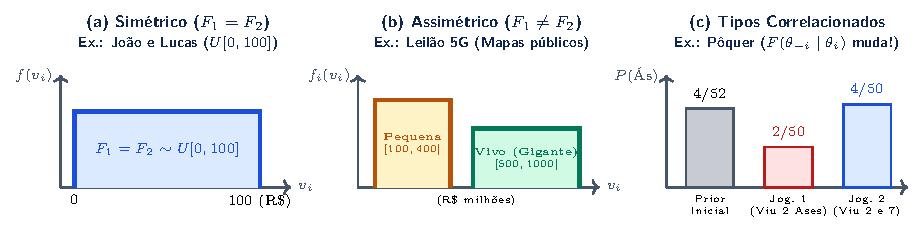
\includegraphics[width=0.80\textwidth]{harsanyi_tipos_prior.pdf}
\end{frame}

% -----------------------------------------------------------------------------
% SLIDE 5: ESTRATÉGIA FUNCIONAL E EQUILÍBRIO DE NASH BAYESIANO (DEF 5 E DEF 6)
% -----------------------------------------------------------------------------
\begin{frame}{1.3. Estratégia como Função e Equilíbrio de Nash Bayesiano (ENB)}
  \begin{columns}[T, onlytextwidth]
    \begin{column}{0.57\textwidth}
      \defbox{Definição 5 --- Estratégia em um Jogo Bayesiano
      ($b_i(\theta_i)$)}{%
        Em um jogo bayesiano, uma estratégia \textbf{não é uma única
        ação isolada}, mas sim um \textbf{plano completo (uma função
        matemática)} que especifica qual ação (lance) o jogador $i$
        escolherá \textbf{para cada Tipo $\theta_i$ que a Natureza
        possa ter sorteado para ele} (GIBBONS, 1992).
      }
      \vspace{0.08cm}
      \defbox{Definição 6 --- Equilíbrio de Nash Bayesiano (ENB)}{%
        É um perfil de funções de estratégia
        $\big(b_1^\ast(\theta_1), \dots, b_n^\ast(\theta_n)\big)$ ---
        uma regra de lance para cada jogador --- tal que, para todo
        jogador $i$ e para todo Tipo possível $\theta_i$ desse
        jogador, o lance $b_i^\ast(\theta_i)$ maximiza o
        \textbf{ganho médio esperado} de $i$ (calculado sobre a
          distribuição de tipos dos adversários $F(\theta_{-i} \mid
        \theta_i)$), dado que todos os outros jogadores estão usando
        as funções de lance $b_{-i}^\ast(\theta_{-i})$.
      }
    \end{column}
    \begin{column}{0.40\textwidth}
      \exbox{Intuição-Chave}{%
      \begin{itemize}\setlength{\itemsep}{3pt}
          \item \textbf{Notação ``$-i$'':} Todos os jogadores exceto
            $i$ (com $n=2$, $\theta_{-1} = \theta_2$).
          \item \textbf{Ótimo para todo tipo SEU ($\theta_i$):} Você
            já sabe seu próprio $\theta_i$ ao preencher o envelope!
          \item \textbf{Ótimo EM MÉDIA sobre $\theta_{-i}$:} No 1º
            Preço ($b^\ast(v_i)=v_i/2$), você maximiza a esperança
            (\textit{interim}); no 2º Preço ($b^\ast(v_i)=v_i$), é
            ótimo até \textit{ex post}!
          \item \textbf{Analogia da Calculadora de Vidro:} Todos
            conhecem a \textbf{fórmula} do rival
            ($b_2^\ast(v_2)=v_2/2$), mas não o \textbf{número $v_2$}
            digitado hoje!
        \end{itemize}
      }
    \end{column}
  \end{columns}
\end{frame}

% -----------------------------------------------------------------------------
% SLIDE 6: VALORAÇÃO, VALORES PRIVADOS (IPV) E VALOR COMUM (CV) (DEF 7, 8 E 9)
% -----------------------------------------------------------------------------
\begin{frame}{1.4. Ambientes de Leilão: Valores Privados (IPV)
  vs.\ Valor Comum (CV)}
  \defbox{Definição 7 --- Valoração ($v_i$) e Excedente /
  \textit{Payoff} ($u_i$)}{%
    A \textbf{Valoração ($v_i$)} é o valor monetário máximo que o
    objeto leiloado tem para o jogador $i$ (sua disposição máxima a
    pagar). Se o jogador $i$ vence o leilão e paga um preço $p$, o
    seu ganho líquido (\textbf{Excedente do Comprador} ou
    \textbf{\textit{Payoff}}) é $u_i = v_i - p$. Se perde o leilão e
    não paga nada, seu \textit{payoff} é $u_i = 0$.
  }
  \vspace{-0.1cm}
  \begin{columns}[T, onlytextwidth]
    \begin{column}{0.485\textwidth}
      \defbox{Definição 8 --- Valores Privados Independentes (IPV)}{%
        Ambiente em que: \textbf{(1) Valor Privado ($v_i =
        \theta_i$):} cada jogador $i$ conhece com $100\%$ de certeza
        sua própria Valoração $v_i$; mesmo que descobrisse o Tipo dos
        rivais, isso \textbf{não mudaria em um centavo} o quanto o
        bem vale para ele; e \textbf{(2) Independência:} $v_i$ é
        sorteado independentemente de $v_j$.\\[3pt]
        \textbf{Exemplo:} Camisa autografada do time (vale R\$\,500
        p/ você, mesmo que o vizinho só dê R\$\,20).
      }
    \end{column}
    \begin{column}{0.485\textwidth}
      \teobox{Definição 9 --- Valor Comum Puro (CV)}{%
        Ambiente em que o objeto tem \textbf{o mesmo valor objetivo
        $V$ para todos} ($v_1 = \dots = v_n = V$), mas
        \textbf{ninguém conhece $V$ no momento do leilão}. O Tipo
        ($\theta_i = s_i$) é apenas um \textbf{Sinal Privado} ($s_i =
        V + \varepsilon_i$). Se um jogador descobrisse o sinal dos
        rivais, \textbf{mudaria imediatamente sua estimativa}!\\[3pt]
        \textbf{Exemplo:} Petróleo no pré-sal (laudos sísmicos:
        $1{,}2$ bi vs.\ $0{,}8$ bi e $0{,}7$ bi).
      }
    \end{column}
  \end{columns}
\end{frame}

% -----------------------------------------------------------------------------
% SLIDE 7: OS QUATRO FORMATOS CLÁSSICOS E EQUIVALÊNCIAS ESTRATÉGICAS
% -----------------------------------------------------------------------------
\begin{frame}{1.5. Os Quatro Formatos Clássicos e Equivalências Estratégicas}
  \footnotesize
  \begin{table}
    \centering
    \begin{tabular}{p{4.3cm} p{9.8cm}}
      \toprule
      \textbf{Formato de Leilão} & \textbf{Regra de Alocação e
      Pagamento (VICKREY, 1961; KLEMPERER, 2004)} \\
      \midrule
      \textbf{1. Ascendente Aberto (Inglês)} & Preço sobe (viva-voz
      ou relógio c/ mãos levantadas). Vence o último a ficar, pagando
      o preço em que o penúltimo desistiu. \\
      \textbf{2. Descendente Aberto (Holandês)} & Relógio começa alto
      e cai. O 1º a gritar ``Pare!'' vence na hora e paga o preço
      marcado no relógio. \\
      \textbf{3. 1º Preço (Envelope Fechado)} & Cada um entrega lance
      secreto $b_i$. Maior lance vence e \textbf{paga o próprio lance
      ($p = b_i$)}. \\
      \textbf{4. 2º Preço / Vickrey (Fechado)} & Cada um entrega
      lance secreto $b_i$. Maior lance vence, mas \textbf{paga o 2º
      maior lance ($p = \max_{j \neq i} b_j$)}. \\
      \bottomrule
    \end{tabular}
  \end{table}
  \vspace{-0.15cm}
  \begin{columns}[T, onlytextwidth]
    \begin{column}{0.485\textwidth}
      \exbox{Equivalência 1: Holandês $\equiv$ 1º Preço (Sempre!)}{%
        No relógio descendente, ninguém observa nada até alguém
        apertar o botão e encerrar o jogo. Escolher o ponto de parada
        é \textbf{100\% isomorfo} a escrever o lance num envelope
        fechado de 1º Preço!
      }
    \end{column}
    \begin{column}{0.485\textwidth}
      \exbox{Equivalência 2: Inglês $\equiv$ 2º Preço (Sob IPV!)}{%
        \textbf{Exemplo:} Ana ($50$), Lucas ($80$) e João ($100$).
        Ana sai em $50$; Lucas sai em $80$; João vence pagando
        \textbf{R\$\,80} (o limite do 2º colocado, sem revelar $100$)
        --- idêntico a Vickrey!
      }
    \end{column}
  \end{columns}
\end{frame}

% -----------------------------------------------------------------------------
% SLIDE 8: SOMBREAMENTO DE LANCE (BID SHADING) NO 1º PREÇO (DEF 10)
% -----------------------------------------------------------------------------
\begin{frame}{1.6. Como se Joga o 1º Preço? Sombreamento de Lance
  (\textit{Bid Shading})}
  \defbox{Definição 10 --- Sombreamento de Lance (\textit{Bid Shading})}{%
    É o ato deliberado de submeter um lance \textbf{estritamente
    menor do que a sua verdadeira Valoração} ($b_i < v_i$).
  }
  \vspace{-0.05cm}
  \begin{columns}[T, onlytextwidth]
    \begin{column}{0.53\textwidth}
      \defbox{Por que o \textit{Bid Shading} é Obrigatório no 1º Preço?}{%
        Pela fórmula do \textbf{Valor Esperado do Ganho
        (\textit{Payoff} Esperado)}:
        \[
          \mathbb{E}[u_i(b_i) \mid v_i] = \underbrace{(v_i -
          b_i)}_{\text{Lucro se vencer}} \times
          \underbrace{\mathbb{P}\!\Big(b_i > \max_{j \neq i}
          b_j\Big)}_{\text{Probabilidade de vencer}}
        \]
      \begin{itemize}\setlength{\itemsep}{2pt}
          \item Se ofertar $b_i = v_i \implies (v_i - v_i) = 0
            \implies \textbf{Ganho esperado ZERO!}$
          \item \textbf{Subir o lance ($b_i \uparrow$):} Aumenta a
            chance de vencer, mas diminui o lucro $(v_i - b_i) \downarrow$.
          \item \textbf{Baixar o lance ($b_i \downarrow$):} Aumenta o
            lucro $(v_i - b_i) \uparrow$, mas diminui a chance de vencer.
        \end{itemize}
      }
    \end{column}
    \begin{column}{0.44\textwidth}
      \exbox{Lance Ótimo no Equilíbrio de Nash Bayesiano}{%
        Ao maximizar $\mathbb{E}[u_i(b_i) \mid v_i]$, o lance
        sombreado ótimo é o \textbf{Valor Esperado do maior
          adversário, condicionado a todos os adversários terem valor
        menor que $v_i$}:
        \[
          \boxed{b_{\text{1º Preço}}^\ast(v_i) = \mathbb{E}\!\left[\,
          \max_{j \neq i} v_j \;\middle|\; \max_{j \neq i} v_j < v_i \,\right]}
        \]
      \begin{itemize}\setlength{\itemsep}{2pt}
          \item Para $n=2$ jogadores com valores uniformes em
            $[0,1]$, a média de $v_2 \in [0, v_i]$ é exatamente a
            metade: $b^\ast(v_i) = \dfrac{v_i}{2}$ (\textbf{desconto
            de $50\%$}).
        \end{itemize}
      }
    \end{column}
  \end{columns}
\end{frame}

% -----------------------------------------------------------------------------
% SLIDE 9: REVELAÇÃO SINCERA NO 2º PREÇO / VICKREY (DEF 11)
% -----------------------------------------------------------------------------
\begin{frame}{1.7. Como se Joga o 2º Preço (Vickrey)? Revelação Sincera}
  \defbox{Definição 11 --- Revelação Sincera de Valor
  (\textit{Truthful Bidding})}{%
    É a estratégia na qual o jogador submete um lance
    \textbf{exatamente igual à sua verdadeira Valoração} ($b_i =
    v_i$). No Leilão de 2º Preço, $b_i = v_i$ é uma
    \textbf{Estratégia Fracamente Dominante} (e qualquer estratégia
      mentirosa $b_i \neq v_i$ é uma \textbf{Estratégia Fracamente
      Dominada}, pois nunca gera ganho maior que falar a verdade e gera
    ganho estritamente menor em pelo menos um cenário).
  }
  \vspace{-0.05cm}
  \footnotesize
  \textbf{Por que falar a verdade ($v_1 = \text{R\$\,100}$)?} Você
  \textbf{nunca paga o seu lance $b_1$}, mas sim o lance $M$ do
  adversário! Logo, $b_1 = \text{R\$\,100}$ funciona como um
  \textbf{filtro automático perfeito}: ganha quando $M < 100$ (dá
  lucro) e perde quando $M > 100$ (evita prejuízo):
  \vspace{0.1cm}
  \begin{table}
    \centering
    \scriptsize\setlength{\tabcolsep}{4pt}
    \begin{tabular}{p{2.8cm} p{3.3cm} p{3.6cm} p{3.6cm}}
      \toprule
      \textbf{Envelope do Rival ($M$)} & \textbf{Falar a VERDADE
      ($b_1 = 100$)} & \textbf{MENTIR P/ BAIXO ($b_1 = 70$)} &
      \textbf{MENTIR P/ CIMA ($b_1 = 120$)} \\
      \midrule
      \textbf{Caso 1:} $M = \text{R\$\,50}$ & Ganha, paga R\$\,50
      $\to$ \textbf{$+$R\$\,50} & Ganha, paga R\$\,50 $\to$
      $+$R\$\,50 & Ganha, paga R\$\,50 $\to$ $+$R\$\,50 \\
      \textbf{Caso 2:} $M = \text{R\$\,85}$ & \textbf{Ganha}, paga
      R\$\,85 $\to$ \textbf{$+$R\$\,15} &
      \textcolor{itaRed}{\textbf{PERDE}} ($70<85$) $\to$
      \textcolor{itaRed}{\textbf{R\$\,0 (perdeu 15!)}} & Ganha, paga
      R\$\,85 $\to$ $+$R\$\,15 \\
      \textbf{Caso 3:} $M = \text{R\$\,110}$ & \textbf{Perde}
      ($100<110$) $\to$ \textbf{R\$\,0} & Perde ($70<110$) $\to$
      R\$\,0 & \textcolor{itaRed}{\textbf{GANHA}}, paga R\$\,110
      $\to$ \textcolor{itaRed}{\textbf{$-$R\$\,10 (prej.!)}} \\
      \textbf{Caso 4:} $M = \text{R\$\,130}$ & Perde ($100<130$)
      $\to$ R\$\,0 & Perde ($70<130$) $\to$ R\$\,0 & Perde
      ($120<130$) $\to$ R\$\,0 \\
      \bottomrule
    \end{tabular}
  \end{table}
\end{frame}

% -----------------------------------------------------------------------------
% SLIDE 10: TEOREMA DA EQUIVALÊNCIA DE RECEITA (TEOREMA 1)
% -----------------------------------------------------------------------------
\begin{frame}{1.8. Teorema da Equivalência de Receita (RET)}
  \teobox{Teorema 1 --- Teorema da Equivalência de Receita (VICKREY,
  1961; MYERSON, 1981; KLEMPERER, 2004)}{%
    Considere a venda de um único objeto indivisível entre $n$ jogadores:
  \begin{itemize}\setlength{\itemsep}{1.5pt}
      \item \textbf{Hipóteses:} \textbf{(1) Valores Privados
        Independentes (IPV)} ($v_i$ privado e independente);
        \textbf{(2) Simetria} ($v_1, \dots, v_n$ sorteados da mesma
          distribuição contínua $F(v)$ em $[\underline{v},
        \overline{v}]$); \textbf{(3) Neutralidade ao Risco}
        (maximizam $\mathbb{E}[v_i - p]$); e \textbf{(4) Condições no
        ENB dos formatos comparados:} \textbf{(4a) Alocação
        Eficiente} (vence sempre quem tem o maior $v_i$) e
        \textbf{(4b) Fronteira Inferior} (quem tira $v_i =
        \underline{v}$ tem ganho esperado zero).
      \item \textbf{Consequência (Tese):} \textbf{(i) Mesma Receita
        Esperada:} todos esses mecanismos geram \textbf{exatamente a
        mesma receita média esperada para o vendedor}; e \textbf{(ii)
        Mesmo Pagamento Esperado por Tipo:} cada tipo $v_i$ faz o
        mesmo pagamento esperado em todos eles (Inglês, Holandês, 1º
        Preço e 2º Preço/Vickrey empatam!).
    \end{itemize}
  }
  \vspace{-0.1cm}
  \exbox{Intuição Econômica: O ``Cabo de Guerra'' ($n=2$ jogadores
  uniformes entre R\$\,0 e R\$\,100)}{%
    Em média, o \textbf{1º colocado} vale \textbf{R\$\,66,67} ($2/3$)
    e o \textbf{2º colocado} vale \textbf{R\$\,33,33} ($1/3$):
    \[
      \text{\textbf{1º Preço: }} \underbrace{50\%}_{\text{Bid
      Shading}} \times \underbrace{\text{R\$\,66,67}}_{\text{1º
      colocado}} = \mathbf{\text{R\$\,33,33}}
      \qquad \Longleftrightarrow \qquad
      \text{\textbf{2º Preço: }} \underbrace{100\%}_{\text{Sincero}}
      \times \underbrace{\text{R\$\,33,33}}_{\text{2º colocado}} =
      \mathbf{\text{R\$\,33,33}}
    \]
  }
\end{frame}

% -----------------------------------------------------------------------------
% SLIDE 11: SIMULAÇÃO DE MONTE CARLO E QUEBRAS DO RET
% -----------------------------------------------------------------------------
\begin{frame}{1.9. Validação Computacional (Monte Carlo) e Quebras do RET}
  \begin{columns}[T, onlytextwidth]
    \begin{column}{0.54\textwidth}
      \centering
      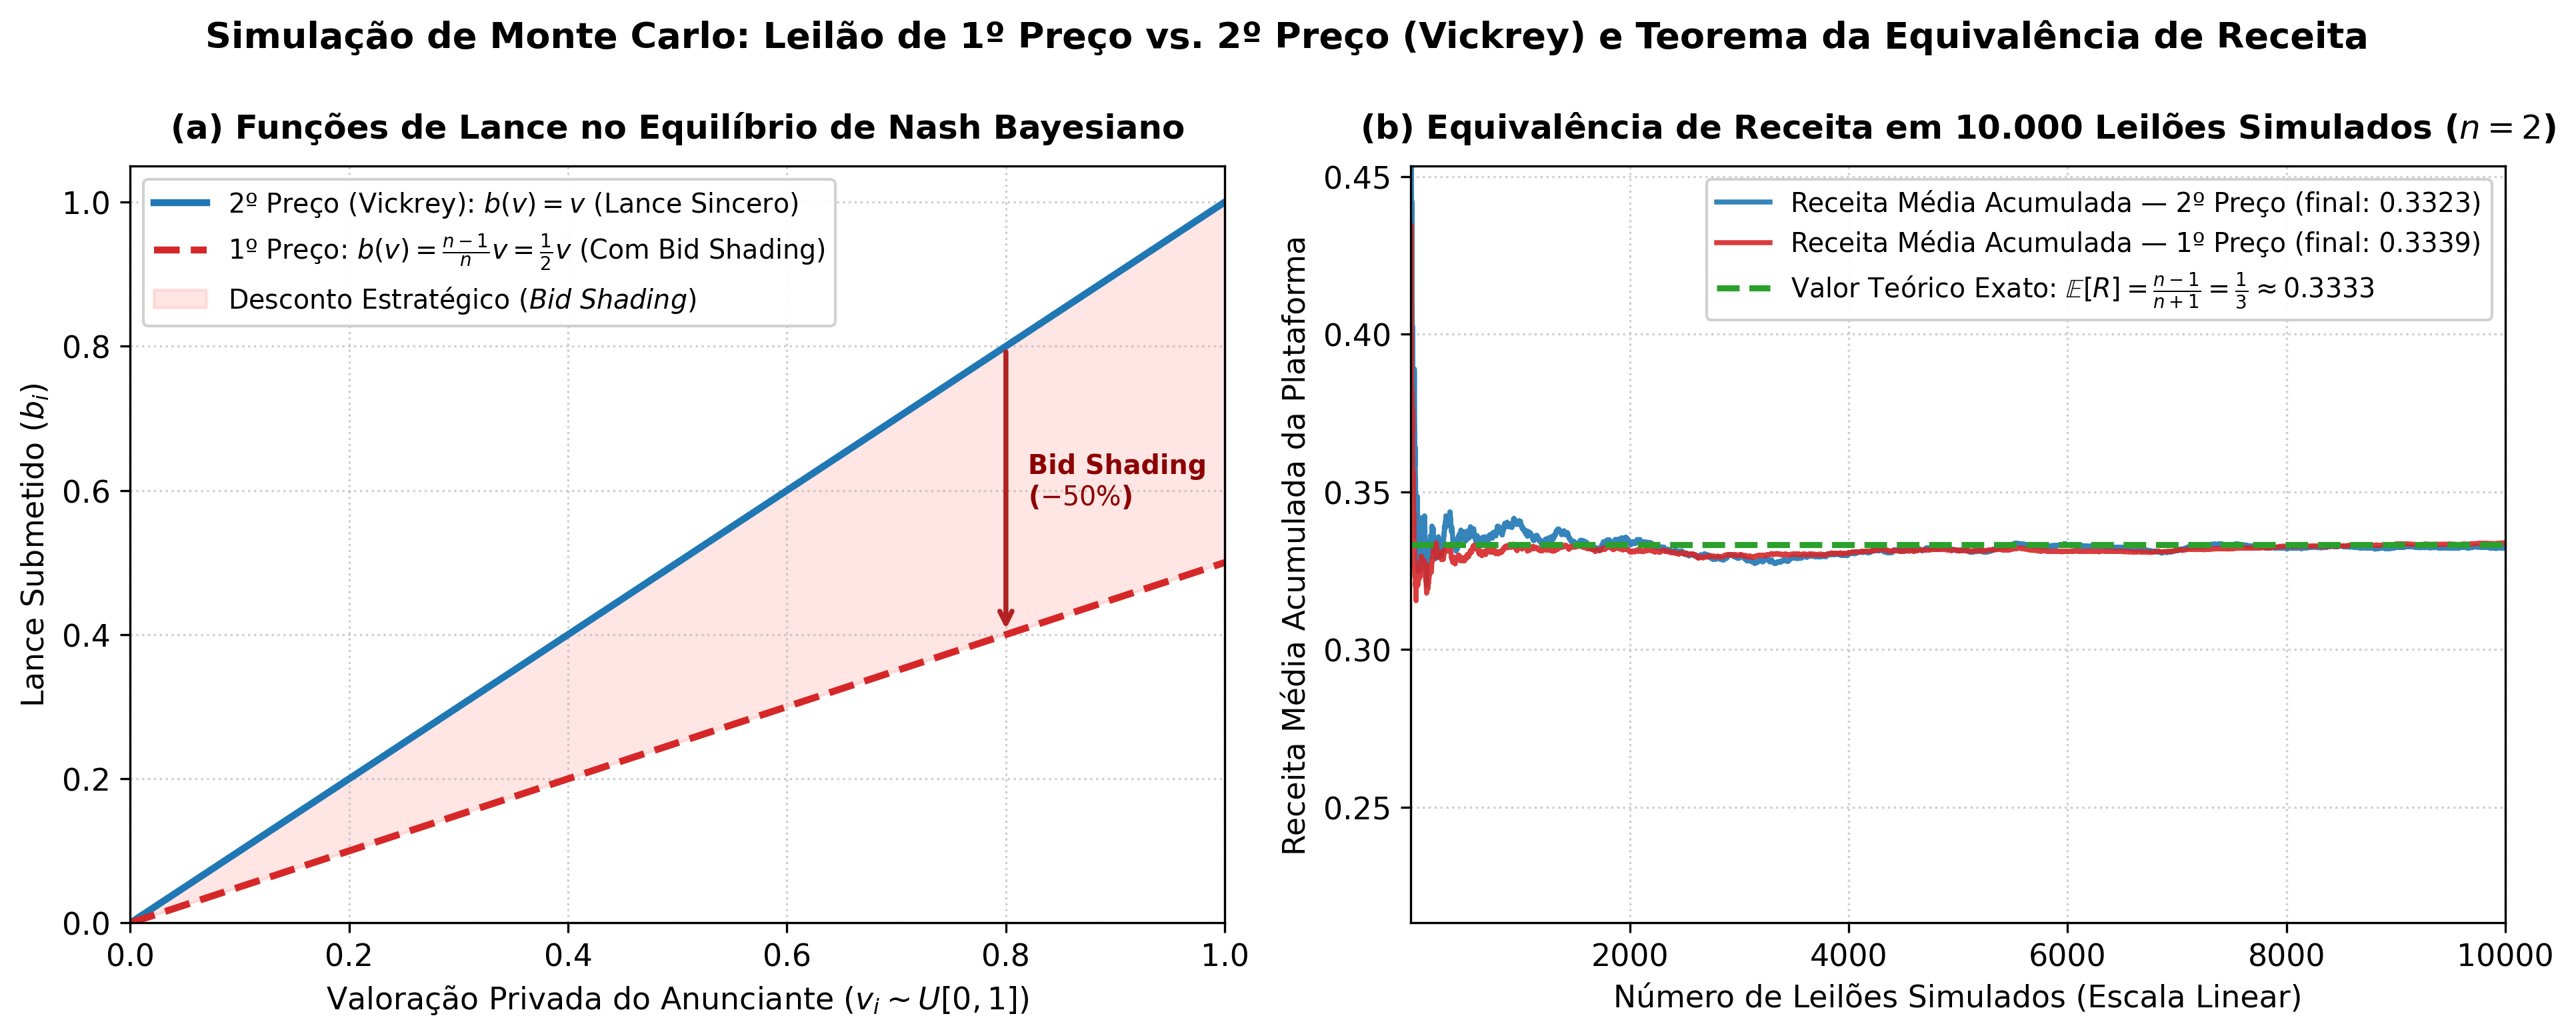
\includegraphics[width=\textwidth]{equivalencia_receita_simulacao.png}
      \vspace{0.05cm}
      \defbox{Simulação de Monte Carlo (\texttt{simulacao\_leilao.py})}{%
        \scriptsize
      \begin{itemize}\setlength{\itemsep}{1.5pt}
          \item $10.000$ leilões simulados com $n=2$ e $v_{t,i} \sim
            U[0,1]$ (semente fixa $= 42$).
          \item \textbf{Receita Média 1º Preço:} $0{,}3339$ (erro $< 0{,}0006$).
          \item \textbf{Receita Média 2º Preço:} $0{,}3323$ (erro $< 0{,}0010$).
          \item \textbf{Valor Teórico Exato (RET):} $\mathbb{E}[R] =
            \frac{n-1}{n+1} = \frac{1}{3} \approx 0{,}3333$.
        \end{itemize}
      }
    \end{column}
    \begin{column}{0.44\textwidth}
      \teobox{Quando o RET Quebra no Mundo Real?}{%
      \begin{enumerate}\setlength{\itemsep}{3pt}
          \item \textbf{Aversão ao Risco (Quebra Hip.\ 3):}
            Compradores têm medo de perder $\to$ descontam menos no
            1º Preço (ex.: dão $70\%$ em vez de $50\%$), mas mantêm
            $b_i=v_i$ no 2º Preço.\\
            $\Rightarrow$ \textbf{Receita(1º Preço) $>$ Receita(2º Preço)!}
          \item \textbf{Assimetria (Quebra Hip.\ 2 --- Ex.\ 5G):}
            Gigante ($[80, 100]$ mi) vs.\ Pequena ($[10, 75]$ mi). No
            2º Preço, a Pequena tem $0\%$ de chance e nem entra; no
            1º Preço, a Gigante faz \textit{shading} (dá R\$\,50 mi)
            e a Pequena pode vencer (dando R\$\,55 mi) $\to$ quebra a
            Eficiência (4a), mas estimula competição!
          \item \textbf{Conluio / Cartel:} 1º Preço fechado dificulta
            fiscalização do cartel $\to$ maior receita.
        \end{enumerate}
      }
    \end{column}
  \end{columns}
\end{frame}

% -----------------------------------------------------------------------------
% SLIDE 12: A MALDIÇÃO DO VENCEDOR (DEF 12)
% -----------------------------------------------------------------------------
\begin{frame}{1.10. A Maldição do Vencedor (\textit{Winner's Curse})}
  \defbox{Definição 12 --- Maldição do Vencedor (\textit{Winner's Curse})}{%
    Em um leilão de \textbf{Valor Comum}, suponha que todos os
    participantes têm estimativas não-viesadas do valor real $V$ (na
      média, a estimativa de todos acerta $V$, mas uns erram para mais
    e outros para menos). Se todos usam a mesma regra de dar lance
    proporcional à sua estimativa, \textbf{quem ganha o leilão não é
      quem fez a estimativa mais precisa, mas sim quem cometeu o maior
    erro de superestimação (o mais otimista da sala)!} Se os
    jogadores não descontarem esse viés ao calcular seus lances, o
    vencedor frequentemente pagará mais do que o objeto realmente
    vale ($p > V$) e terá prejuízo (KLEMPERER, 2004, p.\ 14).
  }
  \vspace{-0.12cm}
  \begin{columns}[T, onlytextwidth]
    \begin{column}{0.38\textwidth}
      \footnotesize
    \begin{itemize}\setlength{\itemsep}{3pt}
        \item \textbf{Analogia do Pote de Moedas:} Pote tem $V =
          \text{R\$\,100}$. Turma chuta na média R\$\,100, mas o mais
          otimista chuta \textbf{R\$\,150}, dá lance de R\$\,130 e
          toma \textbf{prejuízo de R\$\,30}!
        \item \textbf{Como evitar no ENB?} \textbf{Condicionamento na Vitória:}
          \[
            \mathbb{E}\!\left[\, V \;\middle|\; s_i,\; \max_{j \neq
            i} s_j < s_i \,\right]
          \]
          Quanto maior $n$, mais conservador deve ser o lance!
      \end{itemize}
    \end{column}
    \begin{column}{0.60\textwidth}
      \centering
      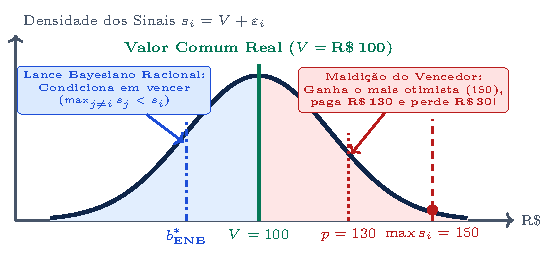
\includegraphics[width=\textwidth]{ipv_vs_cv_maldicao.pdf}
    \end{column}
  \end{columns}
\end{frame}

% =============================================================================
% SEÇÃO 2: MODELO RESOLVIDO PASSO A PASSO
% =============================================================================
\section{Modelo Resolvido Passo a Passo}
\slidesecao{2}{Modelo Resolvido Passo a Passo}{Leilão de 1º Preço
  vs.\ 2º Preço com $n=2$ e $v_i \sim U[0,1]$: Equilíbrio via EDO e
Comparação de Receita}

% -----------------------------------------------------------------------------
% SLIDE 13: ENUNCIADO DO MODELO FORMAL (SEM GRÁFICO)
% -----------------------------------------------------------------------------
\begin{frame}{2.1. Modelo Resolvido: Enunciado e Formulação}
  \defbox{Enunciado do Problema Formal (Grupo 5)}{%
    \textit{``Leilão de primeiro preço com dois participantes e
      valores uniformes entre $0$ e $1$. Derivar o lance de equilíbrio
    e comparar a receita com o leilão de segundo preço.''} (VICKREY,
    1961, p.\ 15--17; KLEMPERER, 2004, Apêndice 1.D, p.\ 48).
  }
  \vspace{0.05cm}
  \begin{columns}[T, onlytextwidth]
    \begin{column}{0.485\textwidth}
      \defbox{Elementos do Jogo Bayesiano}{%
      \begin{itemize}\setlength{\itemsep}{4pt}
          \item \textbf{Jogadores:} $N = \{1, 2\}$ (dois compradores
            simétricos e neutros ao risco).
          \item \textbf{Tipos / Valorações ($v_1, v_2$):} Cada
            jogador $i$ conhece seu valor privado $v_i$, sorteado
            independentemente de $U[0,1]$.
          \item \textbf{Ações:} Lances em envelope fechado $b_1 \ge
            0$ e $b_2 \ge 0$.
          \item \textbf{Objetivo:} Encontrar a função de estratégia
            simétrica de ENB $b_i = \beta(v_i)$, estritamente
            crescente e diferenciável, com $\beta(0) = 0$.
        \end{itemize}
      }
    \end{column}
    \begin{column}{0.485\textwidth}
      \exbox{Propriedade da Uniforme e Regras de Pagamento}{%
      \begin{itemize}\setlength{\itemsep}{4pt}
          \item \textbf{Acumulada da Uniforme em $[0,1]$:} Para
            qualquer número $x \in [0,1]$, a probabilidade de $v_2$
            ser menor que $x$ é o próprio $x$:
            \[
              \boxed{\mathbb{P}(v_2 < x) = F(x) = x}
            \]
          \item \textbf{No 1º Preço:} Quem dá o maior lance vence e
            paga o próprio lance ($p = b_i$).
          \item \textbf{No 2º Preço (Vickrey):} Quem dá o maior lance
            vence e paga o lance do concorrente ($p = b_{-i}$).
        \end{itemize}
      }
    \end{column}
  \end{columns}
\end{frame}

% -----------------------------------------------------------------------------
% SLIDE 14: DERIVAÇÃO DO EQUILÍBRIO NO 1º PREÇO (PASSOS 1 E 2)
% -----------------------------------------------------------------------------
\begin{frame}{2.2. Derivação do Equilíbrio no 1º Preço --- Passos 1 e 2}
  \begin{columns}[T, onlytextwidth]
    \begin{column}{0.54\textwidth}
      \defbox{Passo 1 --- Probabilidade de Vitória do Jogador 1}{%
        Suponha que o Jogador 2 use a estratégia $b_2 = \beta(v_2)$.
        Ao ofertar $b_1 \in [0, \beta(1)]$, o Jogador 1 vence se:
        \[
          \beta(v_2) < b_1 \iff v_2 < \beta^{-1}(b_1)
        \]
        Como $v_2 \sim U[0,1]$ e $0 \le \beta^{-1}(b_1) \le 1$:
        \[
          \boxed{\mathbb{P}\big(\beta(v_2) < b_1\big) =
          \mathbb{P}\big(v_2 < \beta^{-1}(b_1)\big) = \beta^{-1}(b_1)}
        \]
      }
      \defbox{Passo 2 --- Função de \textit{Payoff} Esperado $\Pi_1(b_1)$}{%
        Multiplicando o lucro em caso de vitória $(v_1 - b_1)$ pela
        probabilidade de vencer $\beta^{-1}(b_1)$:
        \[
          \boxed{\Pi_1(b_1) = (v_1 - b_1)\cdot \beta^{-1}(b_1)}
        \]
      }
    \end{column}
    \begin{column}{0.43\textwidth}
      \teobox{Por que ignoramos $b_1 > \beta(1)$ ($\beta^{-1}(b_1) > 1$)?}{%
      \begin{itemize}\setlength{\itemsep}{4pt}
          \item Como $v_2 \le 1$, o \textbf{maior lance possível} do
            Jogador 2 no melhor cenário ($v_2 = 1$) é $\beta(1)$.
          \item Logo, se o Jogador 1 ofertar $b_1 = \beta(1)$, ele
            \textbf{já vence com $100\%$ de certeza ($\mathbb{P} = 1$)}!
          \item Ofertar qualquer $b_1 > \beta(1)$ mantém a chance de
            vitória travada em $100\%$, mas \textbf{paga mais caro à
            toa}, reduzindo o lucro $(v_1 - b_1)$.
          \item Portanto, todo lance $b_1 > \beta(1)$ é
            \textbf{estritamente dominado} por $\beta(1)$.
        \end{itemize}
      }
    \end{column}
  \end{columns}
\end{frame}

% -----------------------------------------------------------------------------
% SLIDE 15: DERIVAÇÃO DO EQUILÍBRIO NO 1º PREÇO (PASSOS 3 E 4)
% -----------------------------------------------------------------------------
\begin{frame}{2.3. Derivação do Equilíbrio no 1º Preço --- Passos 3 e
  4 (CPO e EDO)}
  \begin{columns}[T, onlytextwidth]
    \begin{column}{0.56\textwidth}
      \defbox{Passo 3 --- Condição de Primeira Ordem (CPO)}{%
        Derivando $\Pi_1(b_1) = (v_1 - b_1)\beta^{-1}(b_1)$ em
        relação a $b_1$ (regra do produto):
        \[
          \frac{d\Pi_1}{db_1} = -\beta^{-1}(b_1) + (v_1 -
          b_1)\frac{d}{db_1}\!\big[\beta^{-1}(b_1)\big] = 0
        \]
        No equilíbrio ($b_1 = \beta(v_1)$), $\beta^{-1}(b_1) = v_1$ e
        $\frac{d}{db_1}[\beta^{-1}(b_1)] = \frac{1}{\beta'(v_1)}$:
        \[
          -v_1 + \frac{v_1 - \beta(v_1)}{\beta'(v_1)} = 0 \implies
          \mathbf{v_1 \beta'(v_1) + \beta(v_1) = v_1}
        \]
      }
      \vspace{-0.1cm}
      \defbox{Passo 4 --- Resolução da Equação Diferencial}{%
        Como $\frac{d}{dv_1}[v_1 \beta(v_1)] = v_1 \beta'(v_1) +
        \beta(v_1)$, integrando de $0$ a $v_1$ ($\beta(0)=0$):
        \[
          v_1 \beta(v_1) = \int_0^{v_1} x\,dx = \frac{v_1^2}{2}
          \implies \boxed{b_{\text{1º}}^\ast(v_i) = \beta(v_i) = \frac{v_i}{2}}
        \]
      }
    \end{column}
    \begin{column}{0.41\textwidth}
      \exbox{Generalização para $n$ Jogadores}{%
        Com $n$ jogadores uniformes em $[0,1]$ (VICKREY, 1961, p.\ 17):
        \[
          \boxed{b_{\text{1º}}^\ast(v_i) = \frac{n-1}{n}\,v_i}
        \]
      \begin{itemize}\setlength{\itemsep}{2.5pt}
          \item $n = 2 \implies b^\ast(v_i) = \frac{1}{2}v_i$ ($50\%$ do valor)
          \item $n = 3 \implies b^\ast(v_i) = \frac{2}{3}v_i$
            ($66{,}7\%$ do valor)
          \item $n = 10 \implies b^\ast(v_i) = \frac{9}{10}v_i$
            ($90\%$ do valor)
          \item $n \to \infty \implies b^\ast(v_i) \to v_i$ ($100\%$
            do valor: a concorrência elimina o \textit{bid shading}!)
        \end{itemize}
      }
    \end{column}
  \end{columns}
\end{frame}

% -----------------------------------------------------------------------------
% SLIDE 16: COMPARAÇÃO DE RECEITA ESPERADA (1º PREÇO VS 2º PREÇO + BLOCO FATIAS)
% -----------------------------------------------------------------------------
\begin{frame}{2.4. Comparação da Receita Esperada: 1º Preço vs.\ 2º Preço}
  \begin{columns}[T, onlytextwidth]
    \begin{column}{0.49\textwidth}
      \defbox{1. Receita Esperada no 1º Preço ($\mathbb{E}[R_{\text{1º}}]$)}{%
        Vence o maior valor, pagando metade ($R_{\text{1º}} =
        \frac{1}{2}\max\{v_1, v_2\}$).\\
        Acumulada do máximo: $F_{\max}(y) = \mathbb{P}(v_1 \le
        y)\mathbb{P}(v_2 \le y) = y^2$, logo $f_{\max}(y) = 2y$:
        \[
          \mathbb{E}[\max\{v_1, v_2\}] = \int_0^1 y(2y)\,dy = \frac{2}{3}
        \]
        \[
          \boxed{\mathbb{E}[R_{\text{1º}}] =
          \frac{1}{2}\times\frac{2}{3} = \frac{1}{3}}
        \]
      }
    \end{column}
    \begin{column}{0.49\textwidth}
      \defbox{2. Receita Esperada no 2º Preço / Vickrey
      ($\mathbb{E}[R_{\text{2º}}]$)}{%
        Estratégia dominante: $b^\ast(v_i) = v_i$. Vencedor paga o 2º
        colocado ($R_{\text{2º}} = \min\{v_1, v_2\}$). Como $\min +
        \max = v_1 + v_2$:
        \[
          \mathbb{E}[\min\{v_1, v_2\}] = \mathbb{E}[v_1 + v_2] -
          \mathbb{E}[\max\{v_1, v_2\}] = 1 - \frac{2}{3} = \frac{1}{3}
        \]
        \[
          \boxed{\mathbb{E}[R_{\text{2º}}] = \frac{1}{3} =
          \mathbb{E}[R_{\text{1º}}]}
        \]
      }
    \end{column}
  \end{columns}
  \vspace{0.05cm}
  \exbox{Intuição das Fatias do Intervalo $[0,1]$ (KLEMPERER, 2004, p.\ 48)}{%
    Quando sorteamos $n$ números uniformemente entre $0$ e $1$, eles
    dividem o segmento $[0,1]$ em $n+1$ pedaços iguais em média. Para
    $n=2$ jogadores, os dois valores sorteados dividem $[0,1]$ em 3
    terços: o menor valor ($\min\{v_1, v_2\}$) cai em média em $1/3$,
    e o maior valor ($\max\{v_1, v_2\}$) cai em média em $2/3$. No
    \textbf{2º Preço}, o vendedor recebe o menor valor ($1/3$); no
    \textbf{1º Preço}, recebe metade do maior valor ($\frac{1}{2}
    \times \frac{2}{3} = 1/3$). \textbf{Ambos geram $1/3$!}
  }
\end{frame}

% =============================================================================
% SEÇÃO 3: CASO REAL
% =============================================================================
\section{Caso Real: Leilões de Anúncios Online}
\slidesecao{3}{Caso Real: Leilões de Anúncios Online}{Google Ads e
  \textit{Ad Exchanges}: Evolução (1º $\to$ 2º $\to$ 1º Preço),
\textit{Header Bidding} e Modelagem Bayesiana}

% -----------------------------------------------------------------------------
% SLIDE 17: CASO REAL — ANÚNCIOS ONLINE (GRÁFICO DENTE DE SERRA CENTRALIZADO)
% -----------------------------------------------------------------------------
\begin{frame}{3.1. Caso Real: Anúncios Online e a Mudança de 2002 (1º
  $\to$ 2º Preço)}
  \begin{columns}[T, onlytextwidth]
    \begin{column}{0.46\textwidth}
      \defbox{Conceitos Básicos de Publicidade Digital}{%
        \scriptsize
      \begin{itemize}\setlength{\itemsep}{1.5pt}
          \item \textbf{Impressão:} Exibição de um anúncio ($< 100$ ms).
          \item \textbf{CTR (\textit{Click-Through Rate}):}
            Probabilidade de clique se exibido (ex.: $5\%$).
          \item \textbf{CPC / CPM:} Pagamento por clique vs.\ por mil exibições.
        \end{itemize}
      }
    \end{column}
    \begin{column}{0.52\textwidth}
      \teobox{Fase 1 (1997--2002): ``Dente de Serra'' $\to$ 2º Preço}{%
        \scriptsize
      \begin{itemize}\setlength{\itemsep}{1.5pt}
          \item \textbf{1997 (\textit{Overture} --- 1º Preço
            Visível):} Nike ($v = \text{R\$\,10}$) vs.\ Adidas ($v =
            \text{R\$\,5}$). Robôs subiam de R\$\,0,01 em R\$\,0,01
            até R\$\,5,01, caíam p/ R\$\,1,00 e reiniciavam!
          \item \textbf{2002 (Google 2º Preço):} Cobra R\$\,5,01
            automaticamente (EDELMAN et al., 2007).
        \end{itemize}
      }
    \end{column}
  \end{columns}
  \vspace{-0.05cm}
  \centering
  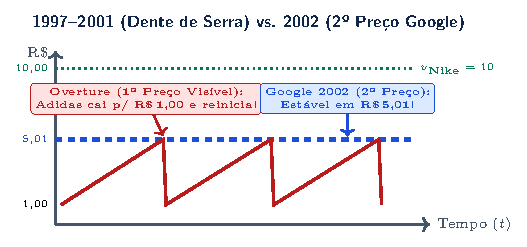
\includegraphics[width=0.58\textwidth]{caso_real_dente_serra.pdf}
\end{frame}

% -----------------------------------------------------------------------------
% SLIDE 18: A SEGUNDA MUDANÇA (2019): IMAGEM CENTRALIZADA
% -----------------------------------------------------------------------------
\begin{frame}{3.2. A Mudança de 2019: Por que o Mercado Voltou do 2º
  para o 1º Preço?}
  \begin{columns}[T, onlytextwidth]
    \begin{column}{0.48\textwidth}
      \teobox{Motivo 1 --- ``Trapaça do Leiloeiro'' (\textit{Soft Floors})}{%
        \scriptsize
      \begin{itemize}\setlength{\itemsep}{1.5pt}
          \item Nike dá \textbf{R\$\,10,00} (sincero) e Adidas dá
            \textbf{R\$\,2,00}.
          \item Corretora espiava o envelope e criava ``piso oculto''
            de \textbf{R\$\,8,50}!
          \item \textbf{No 1º Preço:} Paga exatamente o lance escrito.
        \end{itemize}
      }
    \end{column}
    \begin{column}{0.50\textwidth}
      \exbox{Motivo 2 --- \textit{Header Bidding} (DESPOTAKIS et al., 2021)}{%
        \scriptsize
      \begin{itemize}\setlength{\itemsep}{1.5pt}
          \item \textbf{Corretora A (2º Preço):} Nike (R\$\,10) cai
            cedo p/ \textbf{R\$\,2,00}.
          \item \textbf{Final vs.\ Puma (R\$\,6 na B):} Puma derrota Nike!
          \item \textbf{2019 (1º Preço + \textit{Shading}):} Nike dá
            R\$\,7 e vence!
        \end{itemize}
      }
    \end{column}
  \end{columns}
  \vspace{-0.05cm}
  \centering
  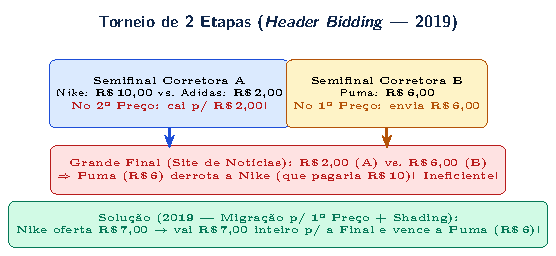
\includegraphics[width=0.60\textwidth]{caso_real_header_bidding.pdf}
\end{frame}

% -----------------------------------------------------------------------------
% SLIDE 19: MODELAGEM FORMAL DO CASO REAL COMO JOGO BAYESIANO
% -----------------------------------------------------------------------------
\begin{frame}{3.3. Modelagem Formal do Caso Real como Jogo Bayesiano}
  \begin{columns}[T, onlytextwidth]
    \begin{column}{0.49\textwidth}
      \defbox{1. Jogadores e 2. Tipos / Informação ($v_i, F$)}{%
      \begin{itemize}\setlength{\itemsep}{3pt}
          \item \textbf{Jogadores:} $N = \{1, \dots, n\}$ anunciantes
            (Nike, Adidas, Puma) disputando a impressão.
          \item \textbf{Tipo Privado ($v_i$):} Valor máximo de 1
            clique. Ex.: Tênis dá \textbf{R\$\,200} de lucro líquido
            e conversão é de $5\%$:
            \[
              v_{\text{Nike}} = 5\% \times \text{R\$\,200} =
              \mathbf{\text{R\$\,10,00 / clique}}
            \]
          \item \textbf{\textit{Prior} Comum ($F$):} Distribuição
            estatística de mercado das valorações do setor.
        \end{itemize}
      }
    \end{column}
    \begin{column}{0.49\textwidth}
      \defbox{3. Estratégias ($b_i(v_i)$) e 4. \textit{Payoffs} ($u_i$)}{%
      \begin{itemize}\setlength{\itemsep}{3pt}
          \item \textbf{Fase 1 (2º Preço):} $b_i^\ast(v_i) = v_i$ (Dominante).
          \item \textbf{Fase 2 (1º Preço pós-2019):} $b_i^\ast(v_i) =
            \frac{n-1}{n}v_i < v_i$ (\textit{Bid Shading} em ENB).
          \item \textbf{\textit{Payoff} por Clique (se $b_i > \max_{j
            \neq i} b_j$):}
            \[
              u_i^{\text{2º}} = v_i - \max_{j \neq i} b_j, \qquad
              u_i^{\text{1º}} = v_i - b_i
            \]
          \item \textbf{Papel do CTR (VARIAN, 2007):}
            $\mathbb{E}[u_i] = \text{CTR} \times (v_i - p) \implies$
            constante positiva não altera o lance ótimo!
        \end{itemize}
      }
    \end{column}
  \end{columns}
\end{frame}

% =============================================================================
% SEÇÃO 4: LIGAÇÃO COM O CURSO GED-62 E CONCLUSÃO
% =============================================================================
\section{Ligação com a Disciplina GED-62 e Conclusões}
\slidesecao{4}{Ligação com a Disciplina GED-62 e Conclusões}{O que os
Leilões Bayesianos acrescentam aos Jogos de Informação Completa e Síntese Final}

% -----------------------------------------------------------------------------
% SLIDE: LIGAÇÃO COM O CURSO GED-62 E CONCLUSÃO (SLIDE EXCLUSIVO)
% -----------------------------------------------------------------------------
\begin{frame}{4. Ligação com o Curso GED-62 e Conclusão}
  \exbox{O que o nosso tema acrescenta a GED-62?}{%
  \begin{enumerate}\setlength{\itemsep}{2pt}
      \item \textbf{Superação da Hipótese de Informação Completa:}
        Nos jogos clássicos (Dilema dos Prisioneiros, Batalha dos
        Sexos, Cournot com custos conhecidos), cada jogador conhece
        os \textit{payoffs} do oponente. Os leilões aplicam a
        Transformação de Harsanyi quando \textbf{há segredo sobre
        quanto o adversário valoriza o prêmio}.
      \item \textbf{Estratégia como Função Contínua ($b_i(v_i)$):} Em
        vez de escolher uma linha ou coluna isolada de uma matriz, a
        estratégia no equilíbrio bayesiano é uma função contínua que
        responde a infinitos tipos possíveis.
      \item \textbf{Contraste entre Dominância e Equilíbrio de Nash
        Bayesiano:} O \textbf{2º Preço (Vickrey)} utiliza
        \textbf{Estratégia Fracamente Dominante} ($b_i = v_i$,
        independente de crenças sobre $F$); já o \textbf{1º Preço}
        exige um \textbf{Equilíbrio de Nash Bayesiano} ($b_i =
        \frac{n-1}{n}v_i$, dependente de $F$).
      \item \textbf{Jogos Dinâmicos vs.\ Estáticos (Equivalência
        Estratégica):} Conecta jogos sequenciais em forma extensiva
        (Inglês e Holandês) com jogos simultâneos em forma normal
        (Envelope Fechado de 2º e 1º Preço).
      \item \textbf{Teoria dos Jogos Reversa (Desenho de
        Mecanismos):} O leiloeiro projeta as regras do jogo (1º
        vs.\ 2º preço, preços de reserva e transparência) para
        induzir eficiência alocativa e maximizar receita.
    \end{enumerate}
  }
  \vspace{-0.12cm}
  \defbox{Síntese Final}{%
    A equivalência teórica entre 1º e 2º Preço ($\mathbb{E}[R] =
    \frac{n-1}{n+1}$) explica o equilíbrio base, enquanto as quebras
    práticas de hipóteses (ciclos dinâmicos em 2002 e torneios de
    múltiplas corretoras no \textit{Header Bidding} em 2019) explicam
    as grandes transformações da indústria digital.
  }
\end{frame}

% -----------------------------------------------------------------------------
% SLIDE 21: REFERÊNCIAS BIBLIOGRÁFICAS (SLIDE EXCLUSIVO)
% -----------------------------------------------------------------------------
\begin{frame}{Referências Bibliográficas (Padrão ABNT)}
  \defbox{Literatura Base e Artigos do Caso Real}{%
    \scriptsize
  \begin{itemize}\setlength{\itemsep}{4pt}
      \item \textbf{DESPOTAKIS, Stylianos; RAVI, R.; SAYEDI, Amin.}
        First-price or second-price? A study of the transition from
        second-price to first-price auctions in online advertising.
        \textbf{Management Science}, Catonsville, v.\ 67, n.\ 10,
        p.\ 6432--6448, out.\ 2021.
      \item \textbf{EDELMAN, Benjamin; OSTROVSKY, Michael; SCHWARZ,
        Michael.} Internet advertising and the generalized
        second-price auction: Selling billions of dollars worth of
        keywords. \textbf{American Economic Review}, Nashville,
        v.\ 97, n.\ 1, p.\ 242--259, mar.\ 2007.
      \item \textbf{GIBBONS, Robert.} \textbf{Game theory for applied
        economists}. Princeton: Princeton University Press, 1992.
      \item \textbf{HARSANYI, John C.} Games with incomplete
        information played by ``Bayesian'' players, I--III: Part I.
        The basic model. \textbf{Management Science}, Catonsville,
        v.\ 14, n.\ 3, p.\ 159--182, nov.\ 1967.
      \item \textbf{KLEMPERER, Paul.} \textbf{Auctions}: theory and
        practice. Princeton: Princeton University Press, 2004.
      \item \textbf{MYERSON, Roger B.} Optimal auction design.
        \textbf{Mathematics of Operations Research}, Catonsville,
        v.\ 6, n.\ 1, p.\ 58--73, fev.\ 1981.
      \item \textbf{VARIAN, Hal R.} Position auctions.
        \textbf{International Journal of Industrial Organization},
        Amsterdã, v.\ 25, n.\ 6, p.\ 1163--1178, dez.\ 2007.
      \item \textbf{VICKREY, William.} Counterspeculation, auctions,
        and competitive sealed tenders. \textbf{The Journal of
        Finance}, Nova York, v.\ 16, n.\ 1, p.\ 8--37, mar.\ 1961.
    \end{itemize}
  }
\end{frame}

\end{document}
